\chapter{Paxos}

In this chapter we provide some background for Paxos and MultiPaxos algorithm. We start with introduction to Paxos and MultiPaxos protocol. Then we describe the problems we encounter while implementing them and performance improvement we made.

\section{Overview}
Paxos algorithm is used to solve consensus problem in distributed system. $n$ processes tries to decide upon the same value, which was proposed by one of them. Paxos is a leader based algorithm so there is always one process, known as leader for majority of processes. The phase of electing the leader is described in following section. When the leader is elected, it starts proposing new values from clients. The MultiPaxos is extension which allows to decide multiple values in specified order instead of just one.

\section{Leader Election}
\label{sec:leader_election}
\indent\par

To decide who is a current leader, our algorithm is using $view$ number. This number is sent in every message and processes keep track of the highest $view$ received. The current leader is a process for which $view \mod n = local\_id$. For example, if $view = 5$ and we have $n = 3$ processes then processes with $local\_id = 2$ is a current leader.

To detect if a leader is correct, failure detector is used. In JPaxos this is done using heartbeats sent periodically by the leader to all processes. The heartbeats are sent only when there are no other messages being sent, that is, the leader sends an \alive message to the replicas if it hasn't sent any message during the last $\tau_0$ time.

When a replica does not receive a message from the leader for more than $\tau_1$ time, it suspects the leader and tries to become the new leader. It advances to the next view where it is the leader and sends a \prepare message to all. For example, if $view = 5$, $n = 3$ and we are process with $local\_id = 1$, we will advance $view$ to number 7 - first view where process 1 is a leader.

To become a leader, process need to prepare the view. It sends the \prepare message to all processes with it's new $view$. Every process which received this message, advances its $view$ and responds with \prepareOK. When a process receives majority of \prepareOK message, it becomes a leader.

\section{Propose Phase}

Every process keeps track of already proposed / decided values in a log. A log is ordered list of consensus instances - triple $<$id, view, value$>$. When a process is a leader, it can start a propose phase for new value. To propose a value, leader creates new consensus instance with first available id, current view and value to propose. Then it is send to all processes in \propose message. Every process when receives the \propose message, saves it to local log and sends \accept message to all. When process receives the majority of \accept message, it will decided the proposed message (and value decided can be later executed on state machine). 

\section{Concurrent instances}
\label{subsec:concurrent_instances}
Running multiple consensus instances simultaneously is an easy way of making the MultiPaxos algorithm faster. Usually, single instance at time is not able to use available bandwidth; running more makes it possible to use the network more efficiently.

Theoretically, we may have any number of concurrent instances active at the same time. We can execute some decision only after all decisions from all instances with lower number have been executed.

In practical approach, the number of instances must be bounded due to following reasons:
\begin{itemize} 
  \item after leader change, \prepareOK must contain all leader's undecided instances,
  \item network has limited bandwidth, and conducting more instances will not increase throughput,
  \item there is no gain if we have decisions for some future instances, but the decision for an instance with lowest ID has not been taken yet (we can neither respond to the client, nor execute the taken decisions),
  \item using UDP, more concurrent instances are causing network congestion so packets are dropped by the system and instances are decided slower.
\end{itemize}

Biggest problem connected with concurrent instances is possibility of ordering the same request twice. Example scenarios explaining the problem:
\begin{figure*}[ht]
  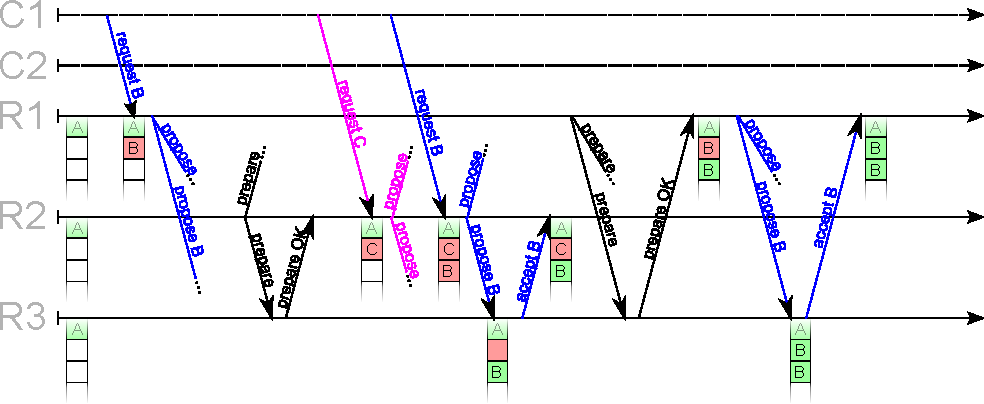
\includegraphics[keepaspectratio, width=\textwidth]{paxos/duplicating_messages.pdf}
  \caption{Duplicating messages - Scenario 1}
\end{figure*}
\begin{description}
  \item [Scenario 1] $R_1$ is the leader, proposes (1:B). No other processes receives these messages and $R_2$ becomes the leader. $R_2$ proposes (1:C) and (2:B). (2:B) is decided. $R_2$ fails and $R_1$ becomes the leader again. While preparing, it learns about (2:B). It has (1:B) as a previously accepted value. The Paxos algorithm requires $R_1$ to propose (1:B) again, since its the accepted value with the highest timestamp, but this will result in the request being decided twice.

  \item [Scenario 2] After a view change, the new primary will know about any value that might have been decided on a previous instance but it might not know about values that were proposed, accepted by up to a minority of replicas but not decided. Suppose that in instance $i$, process $p_1$ had proposed request $R_1$ which was accepted by a minority of replicas. The new primary, $p_2$ doesn't learn about request $R_1$ so it proposes no-op for instance $i$. More or less at the same time, the client resends the request $R_1$ to the new primary, which proposes it and gets it accepted as instance $i+2$, before the no-op request for instance $i$ being accepted. Process $p_2$ crashes and $p_1$ takes over again. Since $p_2$ didn't manage to get no-op accepted for instance $i$, $p_1$ proposes $R_1$ again which ends up being ordered both as instance $i$ and $i+2$.
\end{description} 

Unfortunately we cannot prevent instances from being decided twice in two different instances. Because of that, only valid solution for this problem is to remember last executed instance for every client and not executing them second time. But this requires to keep a new structure in memory as well as by every snapshot (after recovering from snapshot, this structure has to be loaded too).

Even if we cannot prevent from deciding request twice, we should minimise number of such situations because they slow down the algorithm (we have to send redundant data in each message). Possible solutions to decrease them are listed below:
\begin{itemize}
  \item We can cache last reply for each client, so after receiving the same request we can immediately response.
  \item Do not propose requests which are already decided (they can be discarded when creating new batching to propose). 
  \item Current leader can save which requested was proposed by him (but not decided yet) and also discard them. Because in \prepareOK message we can receive instance values which was unknown, leader has to deserialize them first.
\end{itemize}

\paragraph{Setting the window size}
The windows size specifies how many concurrent instances can be started (it has very similar meaning to window size in TCP protocol). In order to use available resources and keep high responsiveness window size must be set correctly. There is no global, generic solution: every usage needs different setting.

Most important thing is monitoring the network: its usage should be high - but no congestion should occur.
That means, on one side, the window size must be enlarged as long as the links are not full, as on the other side, it must be guaranteed that no message will be delayed or dropped because of network traffic.

As long as these conditions hold, a speed of a single instance remains constant (putting aside CPU time).

If network is overused, the overall throughput may even stay on the same level, but the latency will increase for sure.

Notice that having future decisions instead of the present ones does not change decision count per time period, but causes inefficient task arrival time for state machine, especially if many of them arrive at the same time.

\paragraph{Performance Gains}
Single instance will nearly never use available bandwidth, so conducting concurrent instances will surely speed up JPaxos.

In full-duplex networks, concurrent instances will improve network utilisation, because when the leader is waiting for replies, the network from the leader to the followers is idle, so it can be used to send the next request. 

As already mentioned, this solution will improve latency and throughput. Carefulness is required in order to avoid network saturation, especially the link of the leader which has to carry $2n$ messages for each instance (as opposed to 2 messages for every other link).

\section{No operation command}
\paragraph{Scenario}
Three replica $R1$, $R2$ and $R3$. Replica $R1$ is the leader and propose {1:A} and {2:B}. Value {2:B} was decided by all replicas, but {1:A} propose was lost. $R1$ fails and $R2$ becomes new leader. After preparing $R2$ has a gap in log because no information about instance 1 was received. 

As we can see after prepare phase, leader can have a gap in the log. Without filling this gap, replica cannot execute and propose new values. Because of that new value has to be proposed in this place.

With crash-stop or crash-recovery without stable storage the value may be lost forever. That happens when decision $n+1$ is already decided, and decision $n$ is unknown to all but leader, and the leader fails. As only he got the value, and it has been lost -- either because he is not allowed to recover, or he is recovering without stable storage.

On the other hand, the leader change may happen due to lost \alive message. In this case someone has the value, and it could be used back in the voting. The problem is, how to detect this situation.

The easiest solution is to create new request type called no-op, which is null operation and will be ignored by the replica. It fills the gaps, but is not executed on state machine.

It may be worth considering that the leader can use the gap for some other requests. 

\section{Log handling}

\begin{TODO}
  Do something with crash-model here.
\end{TODO}

The replicated log cannot be allowed to grow forever, it must be bounded in any practical system. After a replica executes some command, it no longer needs the corresponding log entry locally. But other replicas may not have learnt the decision during the normal protocol. In this case, these late replicas need to learn the decision by asking the corresponding log entry from a replica that still has it. This is required for view change and, on the crash-recovery model, for recovery. Snapshotting should also be implemented, as it allows faster recovery and filling missing instances. Also for preserving theoretical correctness by log truncating with limited memory either the snapshot mechanism or determining global commit point is needed. Process of getting lost requests is called ``catch-up'', and is described in section \ref{sec:catch_up}.

As log handling differs a lot by different assumptions about post-crash behaviour, we are going to discuss different cases separately.
We start by studying the problem on the crash-stop model.

\subsection{Crash-stop model}
\label{subsec:crash_stop_model}
In this model, there is no need to preserve the contents of the log on stable storage, since the nodes don't survive a crash.

In particular, the log is kept only on volatile memory and it will be there until the process crashes. Therefore, once a command is written on the log of a replica, it is never lost by the replica. A command can be deleted from the log after being executed by all replicas. The highest instance executed by all replicas is called \emph{global commit point}.

The above rule is not enough to ensure that the log is kept bounded, because a correct replica may be disconnected from the system for an arbitrarily long time. When communication is reestablished, the replica needs to learn about all the decisions taken in the meantime, which are an unbounded number. If one replica crashes, the other replicas have no way of knowing that it is a crash (therefore permanent) and not a disconnection, so they would have to keep the logs forever.

Also, some additional mechanisms need to be implemented in order to know the global commit point.

There are several ways of dealing with the problem. One is to block the system when the log limit is reached until all the replicas are back on-line and the logs can once again be deleted. This will likely require human intervention to recover a failed replica.

There is a better alternative for services whose state can be transferred. We totally abandon global commit point, and introduce the snapshots.

Upon reaching the limit of the log, new snapshot with full state is created and the old logs are truncated even if some replicas don't have them yet. When a replica that is missing old logs rejoins, first last snapshot is transferred, later all the decisions from the top of the log that were not yet applied to the state.

The second solution is preferable if transferring the state is practical as it doesn't block the system in case of crashes.

\subsection{Crash-recovery model}
\paragraphNewline{Recovery without stable storage}
Let us remind You one assumption: to guarantee correctness in crash-recovery model without using stable storage, for every moment there has to be at least majority of replicas up-to-date. With this assumption fulfilled, it is possible for replica to recover from other running replicas after crashing. Otherwise, if all replicas, which decided on some instance crash, then information about the instance will be lost and cannot be recovered.

After crashing, replica has to recover only from others. It can either get all decisions, or the current state from other replica.
It is easy to show that this situation is identical to crash-stop approach. Let's take a look on two scenarios:

%\begin{list}{×}{}
%  \item We do not use the global commit point method. For keeping bounded logs, we use snapshots. All replicas start at the same time. One of them, however, is unable to connect to any other replica for a long time $t$. During this period other replicas take decisions normally. After time $t$ the connection is established.
%  
%  Let's see the state now: no replica has ever crashed, and one replica has empty log. The majority of replicas are up-to-date. No history about the replica's activity is held. From the crash-stop model assumptions we know, that the system must be correct.
%  
%  \item All replicas start at the same time, and decide together. After time $t-1$ one replica crashes, and at time $t$ recovers. The recovered replica has just been started, it does not know it has to recover. It's log is of course empty.
%  
%  One replica has crashed and started again, while others work continuously. We assumed that for every moment there has to be at least majority of replicas up-to-date. Again, there is no history of the run. The situation seen by replicas now is the same as the one above.
%\end{list}

So the crash-recovery model without stable storage is identical to crash-stop as long as the majority is up to date and we assume we must use snapshots, and not global commit point as log truncating method.

\paragraphNewline{Recovery with stable storage}

In this model a processes while recovering must read and apply the stable storage contents before it is allowed to take part in the consensus again.

Keeping all instances in stable storage guarantees correctness in crash-recovery model even if all replicas will crash. After crashing, replica has to load and apply saved logs. Then it can rejoin system and execute catch-up mechanism to learn new instances decided after crash.

As we have to keep all instances, the log stays unbounded. We cannot use global commit point for log truncating, as a replica may crash and has to recover from it's logs afterthen.

Snapshotting is a solution again: keeping all actual (not truncated) instances and snapshot in stable storage guarantees correctness in crash-recovery model even if all replicas will crash. While recovering the replica has to load state from snapshot data (saved in stable storage) and apply saved logs not applied yet. Later it rejoins the system and executes catch-up mechanism.

The size of snapshot is bounded, as the state machine must be implemented with the assumption of bounded memory, and the snapshot may be just the processes memory image. The size of the log is bounded as well - we create new snapshot as log size reaches some limit.


\section{Skipping redundant messages}
Reducing number of messages is one of the most efficient optimisation. In JPaxos we do not send messages to self, also the proposer doesn't send \accept messages.

It has been proven for Paxos consensus algorithm that it minimises the count of messages carrying value (client request in our case). Still, there is nothing said about the additional messages. Some of them may be easily skipped without violating guarantees or adding assumptions.

\paragraphNewline{Sending to self}

Many papers concerning Paxos divide the functions into three groups: proposer, acceptor and learner. Processes or some of their parts act as one of them. In order to communicate they must send messages to each other.

In our program every node consists of a proposer, acceptor as well as learner. In this case there is no need to send messages to self. Especially all send-to-all commands may be replaced by send to others command, as long as the communication with self will be done internally. This skips one \accept and one \propose sent by the leader, and one \accept by all other processes.

This does not influence the performance much, however it is recommended as it decreases system -- especially networking stack -- usage. It also skips a few system calls.

\paragraphNewline{Using {\normalfont\propose}as {\normalfont\accept}}

More important optimisation is merging the role of \accept and \textsc{Propose}. As long as acceptors and proposes do not share the log this is not allowed. But if their knowledge is identical and the leader proposed some value, then he must accept it as well. In most solutions one node acts as proposer and acceptor, and they do share the log.

So in JPaxos each \propose is simultaneously an \accept message. Notice that if the system consists of three nodes every process decides on the value by receiving a valid propose -- he knows that the leader and he himself accept the message. Normally the leader process has to send \propose to all first, later \accept to all. By this optimisation we are required to send the half of messages only.

This is a serious gain, clearly visible during benchmarks.
